%(BEGIN_QUESTION)
% Copyright 2011, Tony R. Kuphaldt, released under the Creative Commons Attribution License (v 1.0)
% This means you may do almost anything with this work of mine, so long as you give me proper credit

Et biprodukt fra {\it kraftprosessen} i papirindustrien, der treflis omdannes til masse, er en væske kalt {\it black liquor}. Denne væsken inneholder mange flyktige svovelforbindelser som hydrogensulfid (H$_{2}$S) og mercaptaner. Begge lukter sterkt, og utslipp til atmosfæren utgjør farlige (eller i det minste sterkt sjenerende) utslipp. Tap av flyktige svovelforbindelser betyr også tap av svovel, som er et råstoff i kraftprosessen.

Disse svovelforbindelsene kan stabiliseres slik at de blir mindre flyktige og lettere å gjenvinne gjennom oksidasjon: ved å eksponere black liquor for ren oksygengass. For å minimere oksygenforbruket måles gassstrømmen proporsjonalt mot væskestrøm i et forholdsreguleringssystem:

$$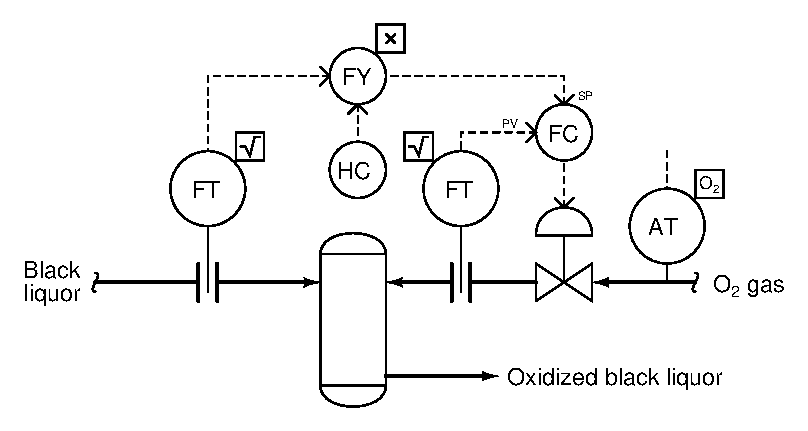
\includegraphics[width=15.5cm]{i00435x01.eps}$$

Ett problem med systemet er at renheten til oksygengassen varierer over tid. Noen dager er den nær 95\% ren, andre dager kan den falle til 80\%. Resten er nitrogengass, som ikke bidrar til oksidasjon av væsken. Driftspersonell oppdaget dette etter at en oksygenanalysator ble installert på O$_{2}$-linjen inn til oksidasjonsreaktoren. Nå ønsker de et reguleringssystem som bruker denne online-målingen og automatisk kompenserer gassstrømmen inn, slik at væsken oksideres riktig uansett oksygenkonsentrasjon.

En nyttig problemløsningsmetode her er et «tankeeksperiment» der oksygenrenheten endres mellom to verdier som er enkle å regne på: anta at renheten starter på 100\%, og plutselig faller til 50\%. Hvordan skal et automatisk kompenseringssystem respondere når O$_{2}$-renheten {\it halveres}, for å opprettholde korrekt oksidasjon av væsken? Bruk deretter denne konklusjonen i en løsning med én eller flere ekstra funksjonsblokker.

\vskip 20pt \vbox{\hrule \hbox{\strut \vrule{} {\bf Forslag til sokratisk diskusjon} \vrule} \hrule}

\begin{itemize}
\item{} Forklar hvordan det foreslåtte tankeeksperimentet gjør dette relativt lett å løse.
\item{} For de som har studert strømningsmåling: forklar hvorfor hver strømningssender har {\it kvadratrottrekk} karakterisering.
\end{itemize}

\underbar{file i00435}
%(END_QUESTION)





%(BEGIN_ANSWER)

Den beste løsningen bruker en {\it divider}-funksjonsblokk i stedet for en summeringsblokk, slik at feedforward-signalet fra oksygenanalysatoren får riktig multiplikativ effekt på oksygenstrømmen til reaktoren dersom oksygenrenheten blir lavere:

$$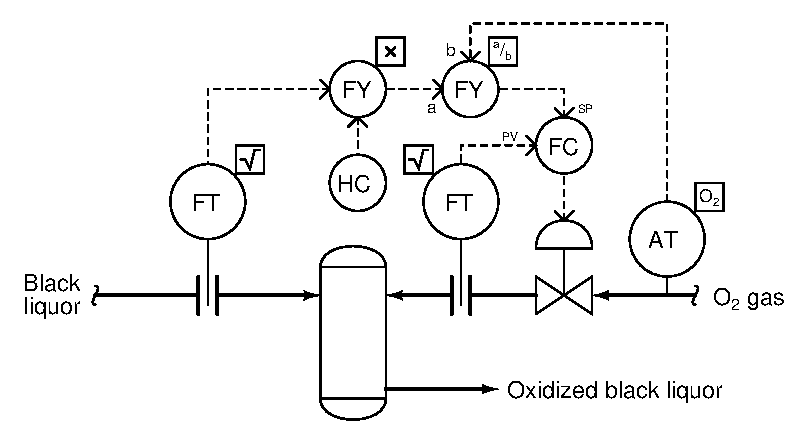
\includegraphics[width=15.5cm]{i00435x02.eps}$$

Hvis oksygenkonsentrasjonen faller fra 100\% til 50\% (for eksempel), trenger vi {\it dobbelt} så høy oksygenstrøm til reaktoren som før, ikke bare et additivt påslag.

%(END_ANSWER)





%(BEGIN_NOTES)


%INDEX% Control, strategies: feedforward
%INDEX% Control, strategies: ratio
%INDEX% Process: black liquor oxidation (Kraft pulping)

%(END_NOTES)
